\documentclass{cubeamer}

\usepackage[french]{babel}
\usepackage[T1]{fontenc}
\usepackage{graphicx}

\title{Protection et gestion des licences}
\subtitle{Présentation - Gestion de projet}
\author{Sami Babigeon, Louka Boivin, Kaci Hammoudi, Alexis Osmont}
\date{\today}
\institute[Université de Rouen]{Master Informatique - 1ère année}

\begin{document}

\maketitle

\cutoc

%   Exemple de plan de présentation (mail de Karim)
%
%   Présentation du sujet et compréhension du besoin client
%   Périmètre fonctionnel à couvrir, appuyé par le diagramme global des cas d’utilisation
%   Solution technique argumentée avec diagramme d’architecture logicielle
%   Stratégie qualité pour la validation des livrables
%   Organisation du projet (i.e. affectation des rôles + découpage des tâches + stratégie de réalisation + organisation agile)
%   Planning du projet (i.e. focus sur les itérations > zoom sur le Gantt)
%   Principaux risques du projet et crédibilité de l'organisation mise en oeuvre
%
%   + POC si on a réussi

\section{Présentation du sujet}

\section{Analyse fonctionnel}

\begin{frame}{Cas d'utilisations}
    \begin{figure}
        \centering
        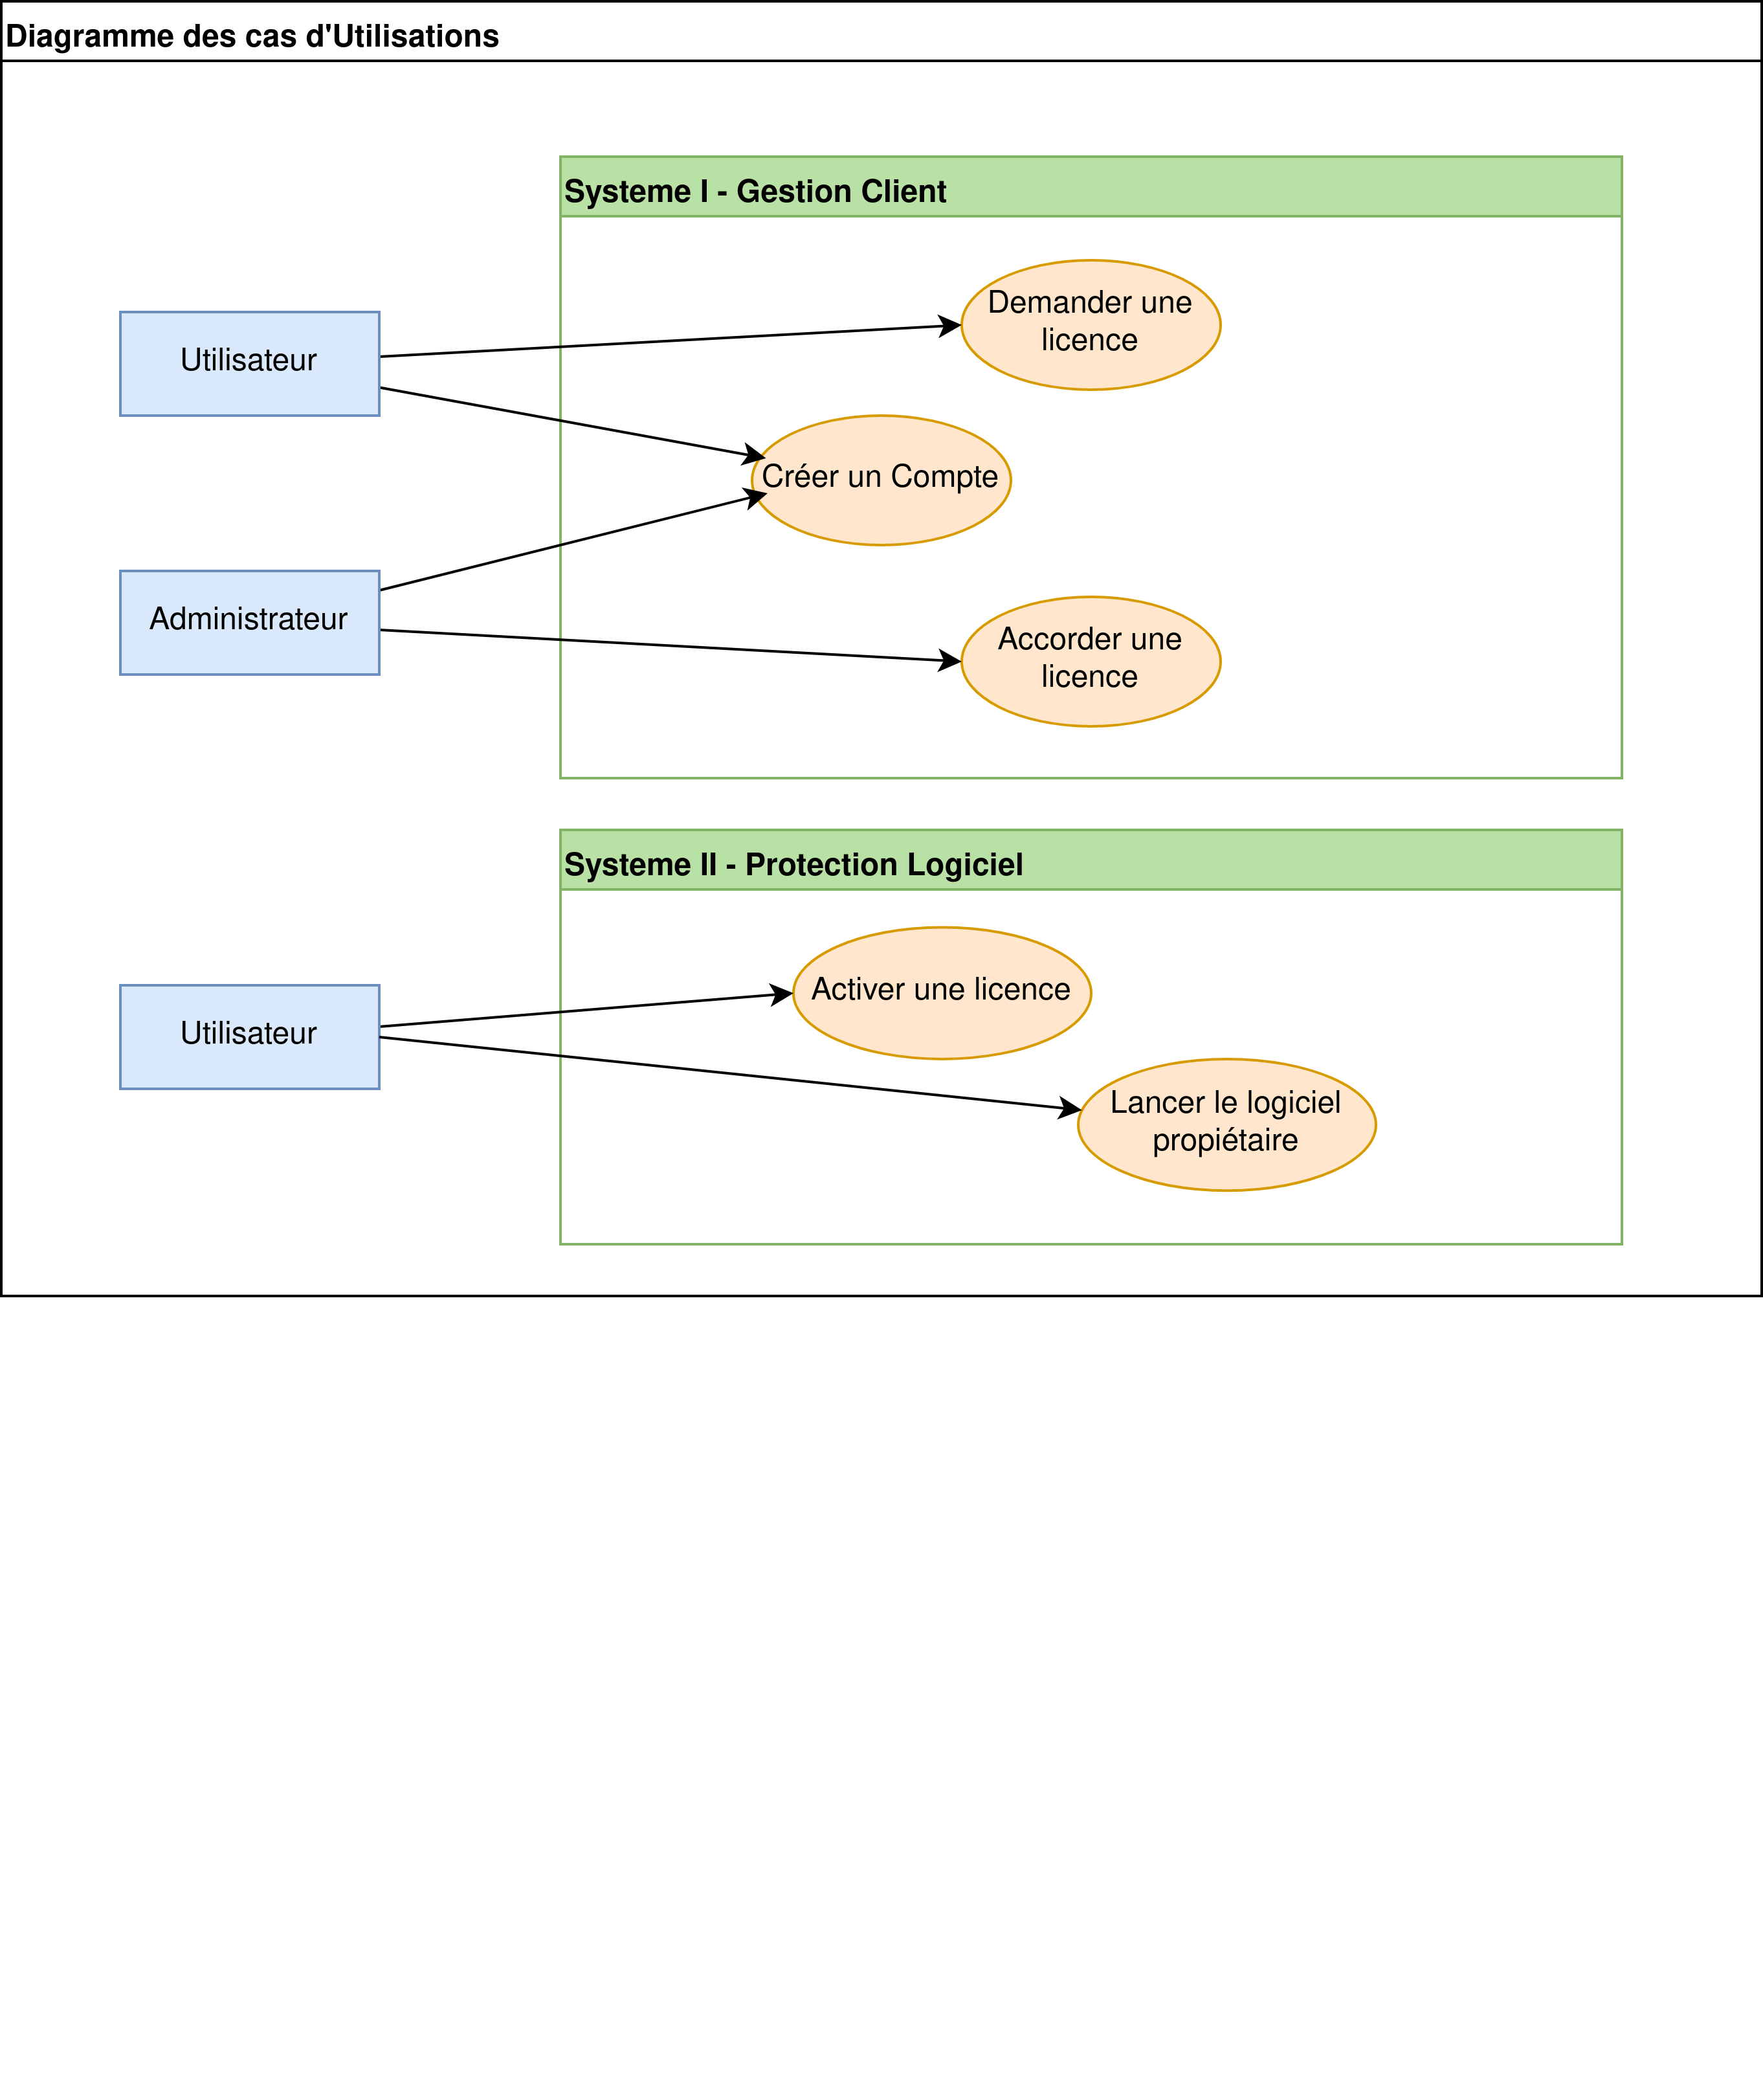
\includegraphics[scale=0.5]{img/Util.png}
    \end{figure}
\end{frame}

\section{Solution technique}

\begin{frame}{Architecture logicielle}
    \begin{figure}
        \centering
        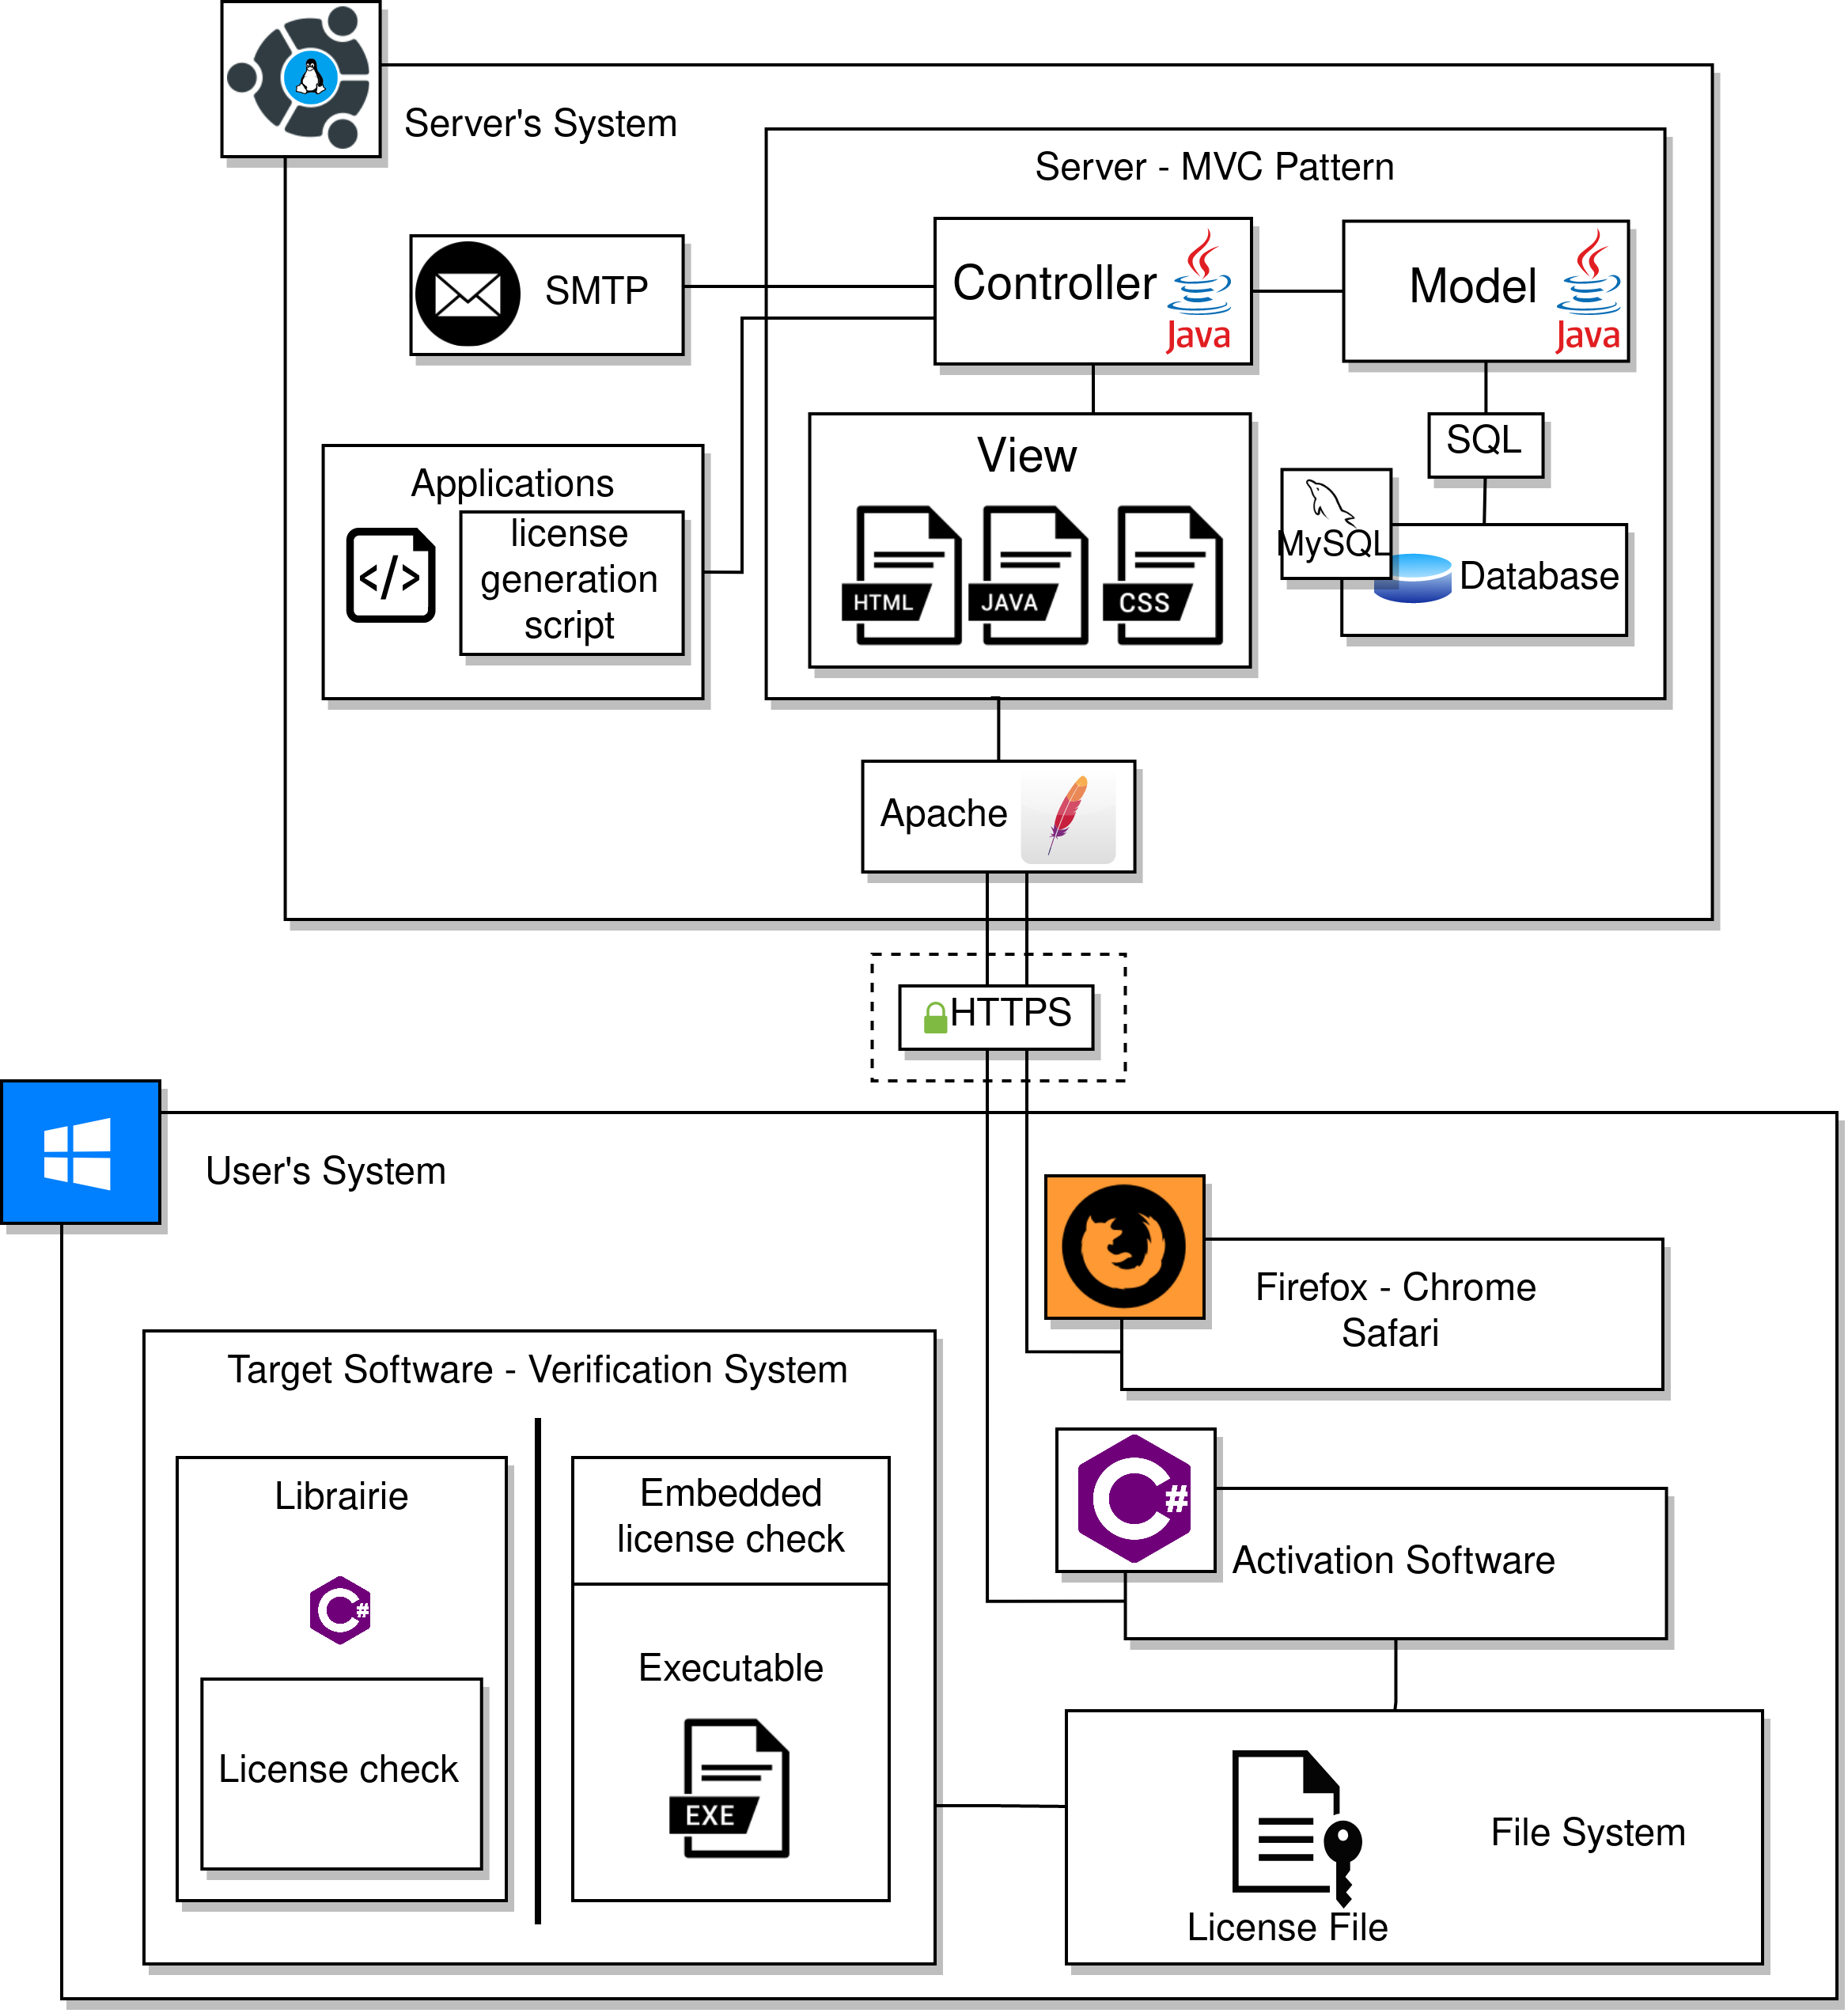
\includegraphics[scale=0.4]{img/DAT_general.png}
    \end{figure}
\end{frame}

\section{Risques}

\section{Stratégie qualité} % en réponse aux risques

\section{Organisation du projet} % + planning

\begin{frame}{Affectation des rôles}
    \begin{figure}
        \centering
        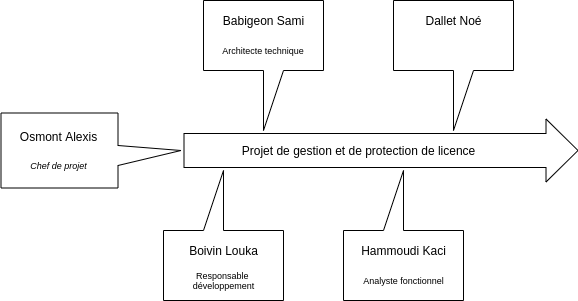
\includegraphics[scale=0.5]{img/schema_role_projet.png}
    \end{figure}
\end{frame}

\begin{frame}{Découpage des tâches}
    \begin{figure}
        \centering
        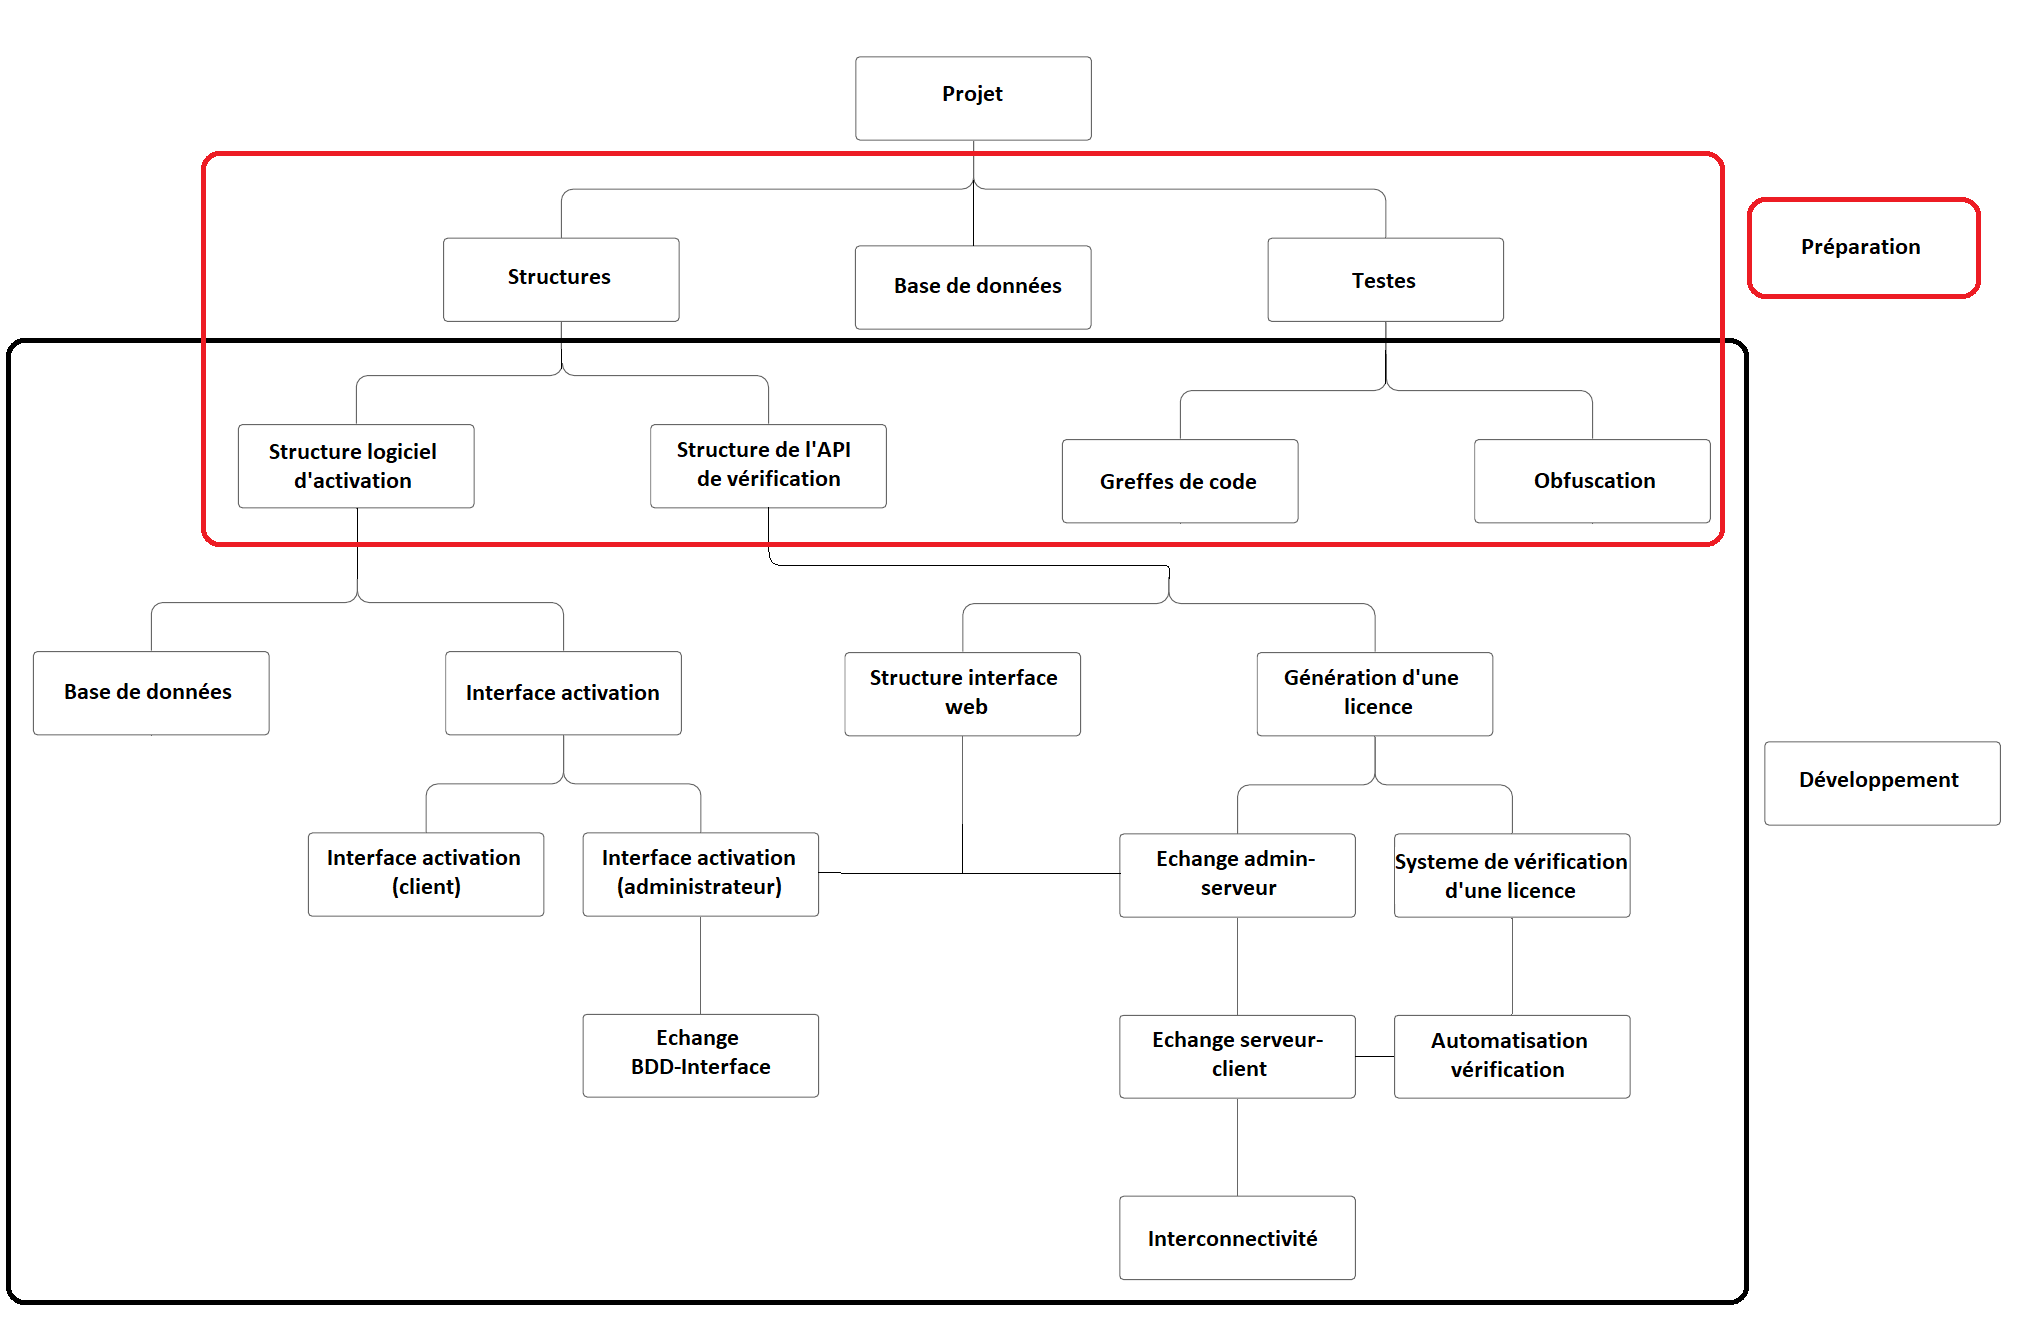
\includegraphics[scale=0.2]{img/organi.png}
    \end{figure}
\end{frame}

\begin{frame}{Diagramme de Gantt}
    \begin{figure}
        \centering
        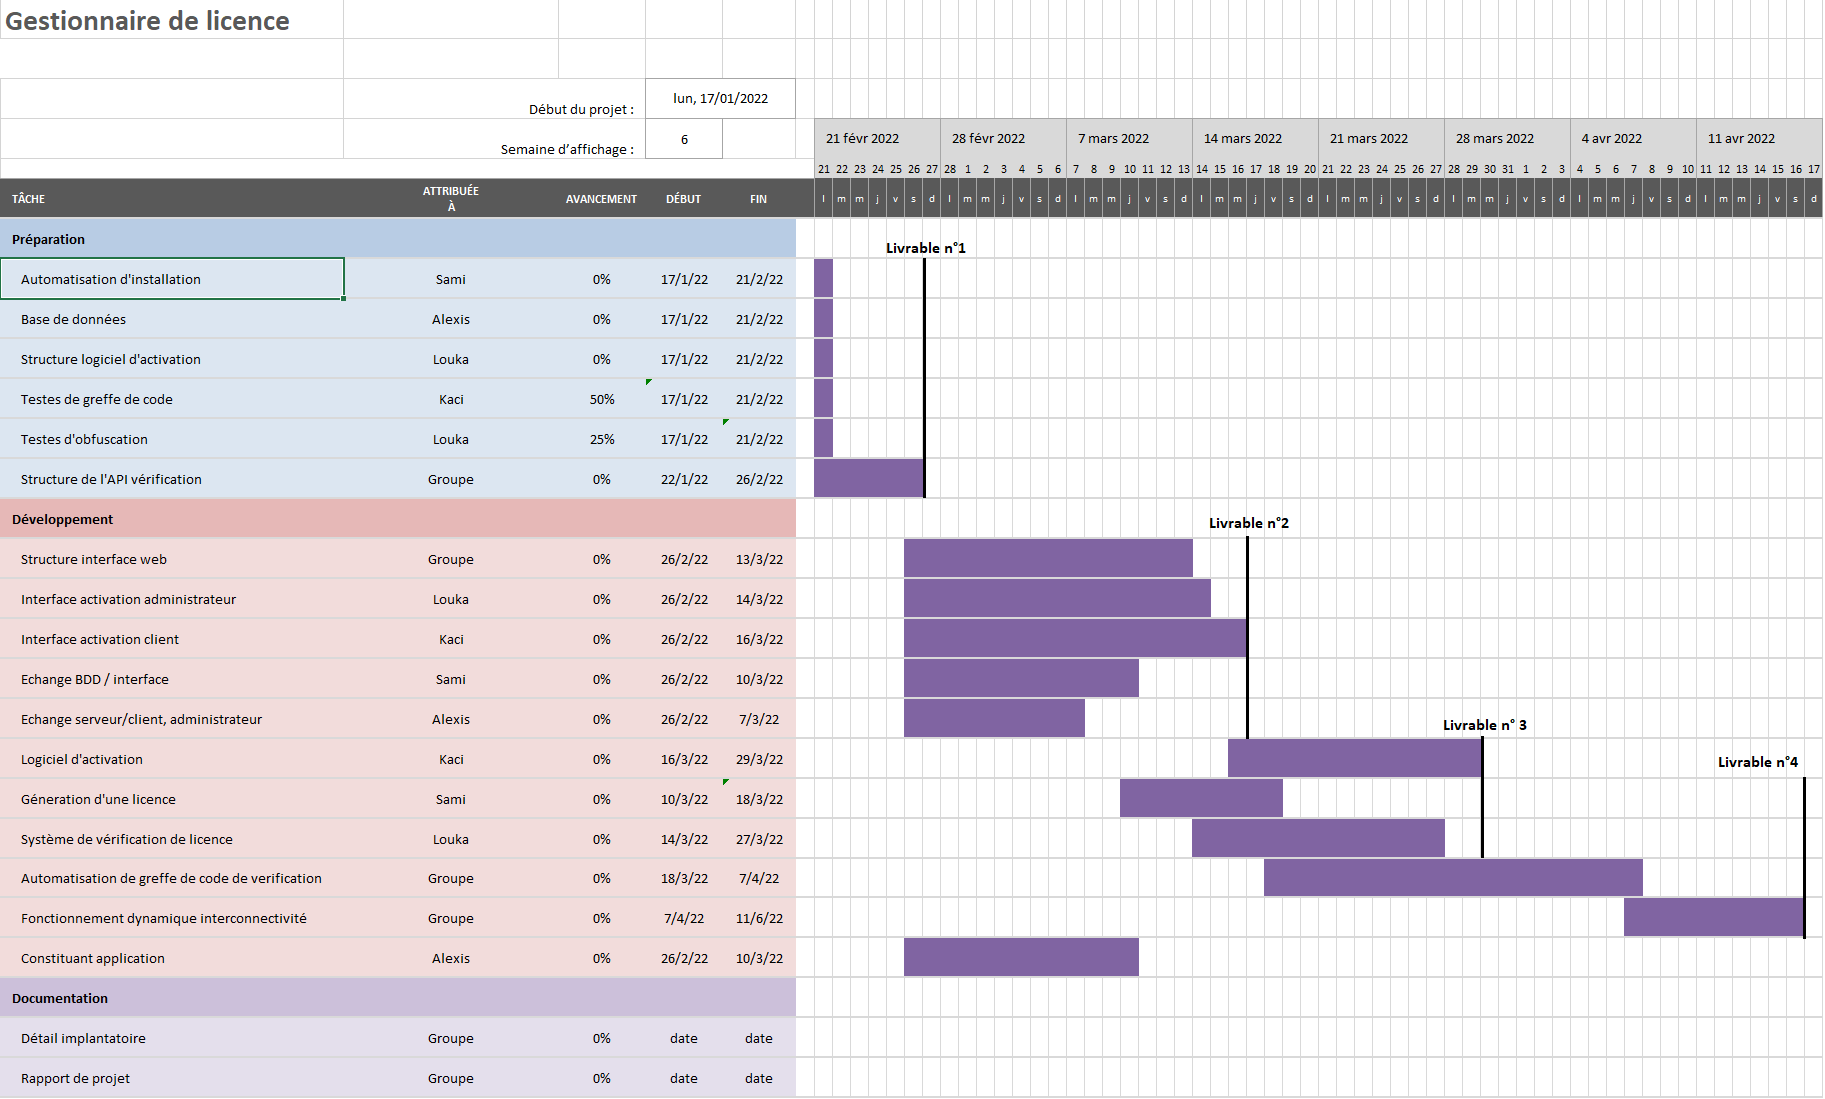
\includegraphics[scale=0.2]{img/Gantt.png}
    \end{figure}
\end{frame}

% Q&A
\begin{frame}[standout]
    \Huge\textsc{Merci de votre écoute}
    \vfill
    \LARGE\textsc{Questions ?}
\end{frame}

\end{document}

